\subsection[]{Dimostrare che all’interno del cono della radiazione Cherenkov vi sono due soluzioni per 
\[
	t'=t-\frac{nR}{c}
,\] 
nessuna soluzione all’esterno, ed una sola sul fronte d’onda.
}\label{sec:4.b.1}
Il problema è stato ampliamente discusso nella spiegazione del fenomeno alla domanda \hyperref[sec:4.a.6]{Domanda 4.a.6}.

\subsection[]{A partire dalla espressione
\[
	\frac{\mbox{d}^2 N_{\gamma}}{\mbox{d}E_{\gamma}\text{d}x} = z^2 \frac{\alpha}{\hbar c}\sin^2\theta_{c}
.\] 
valida per la radiazione Cherenkov, dimostrare che
\[
	N_{\gamma}=z^2 \frac{\alpha}{\hbar c} \int_{E_1}^{E_2}\left[ 1- \frac{1}{\beta^2 \epsilon_{r}\left( E \right)}\right]P_{\text{det}}\left(E\right) dE
.\] 
}\label{sec:4.b.2}
È necessario ricordare, dall'espressione dell'angolo Cherenkov che:
\[
	\sin^2\theta_{c}=1- \frac{c^2}{n^2\left(E\right)v^2}= 1- \frac{1}{\beta^2 \epsilon_{r}\left( E \right) }
.\] 
Successivamente integrando su $x$ si ottiene il fattore $L$ che è la lunghezza del tratto preso in considerazione, integrando anche nell'energia si ottiene anche il fattore $P\left( E \right)$ che è l'efficienza del fotorivelatore.

\subsection[]{Calcolare il numero di fotoni osservati da un fotorivelatore sensibile con efficienza del 30\% a luce fra 300nm e 600nm, al passaggio di un elettrone nei due casi seguenti: \\
	i) n=1.005 (gas), $\beta$=0.999, lunghezza=1m; \\
	ii) n=1.5 (solido trasparente), $\beta$=0.99, lunghezza=1cm.
}\label{sec:4.b.3}
Il conto da fare è l'integrale della espressione nella domanda precedente, il coefficiente di diffrazione è in questo caso indipentente dall'energia, mentre gli estremi di integrazione sono:
\begin{align*}
	&E_1= \hbar \omega_1= \hbar \frac{2\pi c}{\lambda_1} 	&E_2=\hbar \frac{2\pi c}{\lambda_2}
.\end{align*}
Ogni termine può uscire dall'integrale, ne risulta che:
\[
	N_{\gamma}=2\pi \alpha L \left( \frac{1}{\lambda_2}-\frac{1}{\lambda_1} \right) \left( 1- \frac{1}{\beta^2 n^2} \right) P_{\text{det}}
.\] 
Nel primo caso si rilevano 189 fotoni, nel secondo invece se ne rilevano 12533.

\subsection[]{Calcolare l’angolo di emissione della radiazione Cherenkov in funzione dell’impulso (e della massa) della particella e dell’indice di rifrazione.
}
\label{sec:4.b.4}
L'angolo Cherenkov vale \[
	\sin^2\theta_{c}= \frac{1}{n \beta}
.\] 
Sfruttiamo la definizione di $\gamma$ e del'impulso:
\begin{align*}
	&\gamma^2 = \frac{1}{1-\beta^2}		&p = m\gamma v
.\end{align*}
Manipolando le due espressioni si arriva all'equazione:
\[
	\frac{1}{1-\beta^2} = \frac{p^2}{m^2c^2\beta^2}  \implies \beta = \sqrt{\frac{p^2}{p^2+m^2c^2}} 
.\] 
Abbiamo quindi $\beta$ in funzione delle quantità richieste, basta adesso inserire nella prima equazione per concludere:
\[
	\sin^2\theta_{c}=\frac{1}{n} \sqrt{1+\left( \frac{mc}{p} \right)^2} 
.\] 

\subsection[]{Descrivere qualitativamente il principio di funzionamento dei rivelatori Cherenkov: \\
	i) a soglia\\
	ii) RICH\\ 
	iii) DIRC
}
\label{sec:4.b.5}
\paragraph{Rivelatori a soglia.}%
Questi rivelatori sono in grado di rilevare il numero di fotoni emessi ma non l'angolo di emissione.
\begin{figure}[H]
    \centering
    \incfig{rivelatori-checklist-a-soglia}
    \caption{Rivelatori Cherenkov a soglia}
    \label{fig:rivelatori-checklist-a-soglia}
\end{figure}
Il mezzo utilizzato nella camera è un gas ad alta pressione con $n \sim 1.001 - 1.01$, particolarmente adatto a particelle ultrarelativistiche. Questo rilevatore fornisce quindi risposta binaria a seconda che la particella superi o no la velocità della luce nel mezzo:
\begin{itemize}
	\item 0) Se $\beta < 1 /n$
	\item 1) se $\beta > 1 /n$
\end{itemize}
\paragraph{Rivelatore RICH}%
A differenza dei primi questi rivelatori sono in grado di misurare l'angolo di emissione $\theta_{c}$, l'indice di rifrazione del mezzo radiatore è tale da avere solitamente $n < 1.1$, la luce subisce quindi una rifrazione che gli permette comunque di uscire nella stessa direzione della particella (non superando quindi l'angolo limite di riflessione). Tale luce viaggia su superfici coniche e viene osservata su un piano contenente i fotorilevatori, quello che si osserva sono degli anelli: anelli Cherenkov. 
\begin{figure}[H]
	\centering
	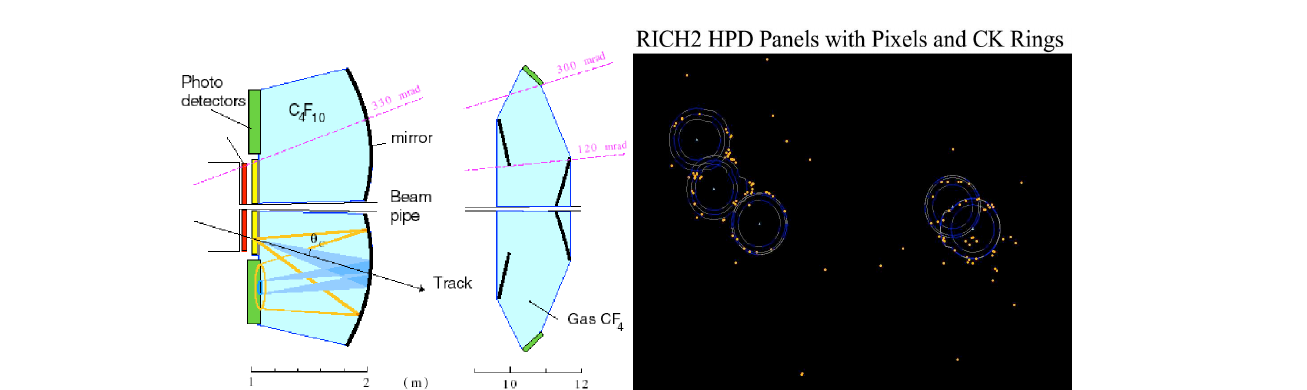
\includegraphics[width=1\textwidth]{immagini/RICH.png}
	\caption{Rilevatore Cherenkov RICH.}
	\label{fig:immagini-RICH-png}
\end{figure}

\paragraph{Rilevatori DIRCH}%
Questo tipo di rivelatore funziona come il Rich: misura l'angolo $\theta_{c}$. L'indice di rifrazione del materiale è solitamente $n\sim 1.4$, per questo la luce viene riflessa internamente fino a raggiungere i lati del radiatore. Per evitare che non esca neanche al lato in cui vorremmo rilevare la radiazione si inserisce un distillato con $n \sim 1.33$ tra radiatore e fotorilevatori.
\begin{figure}[ht]
    \centering
    \incfig{rilevatori-cherenkov-dirch}
    \caption{Rilevatori Cherenkov DIRCH.}
    \label{fig:rilevatori-cherenkov-dirch}
\end{figure}

\subsection[]{Partendo dalla espressione\[
	\frac{\mbox{d} I_{\omega}}{\mbox{d} \Omega} = \frac{q^2}{4\pi^2 c}
	\left|\int\frac{\hat{n}\wedge\left[\left(\hat{n}-\bs{\beta}\right)\wedge\dot{\bs{\beta}}\right]}{\left(1-\hat{n}\cdot\bs{\beta}\right)^2}
	e^{i\omega\left(t'-\frac{\bs{r}'\cdot\hat{n}}{c}\right)}dt'\right|^2.\] 
dimostrare che l’energia persa per unità di frequenza nel caso non relativistico e’ approssimabile con \[
	I_{\omega}=
	\begin{cases}
		\frac{2q^2}{3\pi^2 c}\left| \Delta \bs{\beta} \right|^2  &\text{per } \omega< 1 /\tau\\  
		0 & \text{per } \omega > 1 /\tau
	\end{cases}.\] }
\label{sec:4.b.6}
Nel caso non relativistico la formula di partenza si scrive come :
\[
	\frac{\mbox{d} I_{\omega}}{\mbox{d} \Omega} \approx \frac{q^2}{4\pi^2 c}
	\left|\int\hat{n}\wedge\left[\hat{n}\wedge\dot{\bs{\beta}}\right]
	e^{i\omega t'}dt'\right|^2
.\] 
Se applichiamo questa formula ad una carica non relativistica che si avvicina ad un centro scatterante (nucleo) allora possiamo stimare il tempo di interazione \[
	\tau \approx \frac{b}{v}
.\] 
Con $v$ velocità della particella e $b$ parametro di impatto. Da questo tempo si ricava l'ampiezza di spettro di frequenza ottenibile in trasformata: \[
	\Delta \omega \approx \frac{1}{\tau}
.\] 
Sappiamo quindi che per $\omega\gg \frac{1}{\tau}$ la funzione $\frac{\mbox{d} I_{\omega}}{\mbox{d} \Omega}$ tenderà a zero (lemma di Rieman-Lebesgue), mentre per $\omega\ll \frac{1}{\tau}$ sarà l'espressione scritta sopra integrata nel dominio temporale della intera interazione:\[
	\frac{\mbox{d} I_{\omega}}{\mbox{d} \Omega} \approx 
	\begin{cases}
		\frac{q^2}{4\pi^2 c}
		\left|\int_{- \tau /2}^{\tau /2}\hat{n}\wedge\left[\hat{n}\wedge\dot{\bs{\beta}}\right]
		e^{i\omega t'}dt'\right|^2 		& \text{con } \omega \ll \frac{1}{\tau}\\
		0					& \text{con } \omega \gg \frac{1}{\tau}
	\end{cases}
.\] 
Il modello sussiste quindi nell'approssimare questa funzione con uno scalino "centrato" in $\frac{1}{\tau}$ , sostituiamo l'integrale già svolto:
\[
	\frac{\mbox{d} I_{\omega}}{\mbox{d} \Omega} \approx 
	\begin{cases}
		\frac{q^2}{4\pi^2 c^3} \left| \Delta v \right|^2\sin^2\theta			& \text{con } \omega < \frac{1}{\tau}\\
		0										& \text{con } \omega > \frac{1}{\tau}
	\end{cases}
.\] 
Dove è stato preso un sistema di riferimento in cui $\theta$ è l'angolo tra $\bs{v}$ ed il versore di osservazione del campo $\hat{n}$. \\
Integrando sull'angolo solido si ottiene in fine:
\[
	I_{\omega}=\frac{8}{3}\pi\frac{q^2}{4\pi^2c^3}\left|\Delta v\right|^2\left(1-\theta\left(\omega-\frac{1}{\tau}\right)\right)\theta\left(\omega\right)
.\] 
Che semplificando è l'espressione cercata (in cui si è fatto uso di distribuzioni).

\subsection[]{Partendo dalla espressione \[ 
	\frac{\mbox{d} I_{\omega}}{\mbox{d} \Omega} = \frac{q^2}{4\pi^2 c}
	\left|\int\frac{\hat{n}\wedge\left[\left(\hat{n}-\bs{\beta}\right)\wedge\dot{\bs{\beta}}\right]}{\left(1-\hat{n}\cdot\bs{\beta}\right)^2}
	e^{i\omega\left(t'-\frac{\bs{r}'\cdot\hat{n}}{c}\right)}dt'\right|^2.\] 
dimostrare che l’energia persa per unità di frequenza nel caso non relativistico ad un dato parametro di impatto b è approssimabile con
\[
	I_{\omega}=
	\begin{cases}
		\frac{8z^2Z^2\alpha \hbar c^2}{3\pi}\left( \frac{m_e}{M} \right) ^2 \frac{r^2_e}{V^2}\frac{1}{b ^2} & \text{con } \omega< \frac{V}{b}\\
		0 & \text{con } \omega > \frac{V}{b}
	\end{cases}
.\] 
}
\label{sec:4.b.7}
Si parte in realtà dalla espressione ottenuta nella domanda precedente (all'esame se beccate questa avete già fatto ambo):
\[
	I_{\omega}=
	\begin{cases}
		\frac{2q^2}{3\pi^2 c}\left| \Delta \bs{\beta} \right|  &\text{per } \omega< 1 /\tau\\  
		0 & \text{per } \omega > 1 /\tau
	\end{cases}.
\]
Il prossimo passo è calcolare $\left| \Delta \bs{v} \right| $ in funzione del parametro di impatto $b$, per farlo possiamo approssimare la traiettoria della particella scatterata ad una retta (approssimazione di angoli di scattering piccoli), sempre rispettata sperimentalmente in caso di Bremsstralhung. In questo modo la variazione di quantità di moto è solo perpendicolare alla direzione di incidenza della particella ed il suo modulo è dato da:
\[
	\left| \Delta \bs{p} \right| \approx \left| \int_{\infty}^{\infty} ze \bs{E}_{\bot} dt \right| 
.\] 
Nella approssimazione in cui la velocità della particella risulti invariata:
\[
	\left| \Delta \bs{p} \right| \approx \frac{ze}{v} \left| \int \bs{E}_{\bot} dx\right|= 
	\frac{ze}{2\pi b v} \left| \int 2\pi \bs{E}_{\bot}dx \right|= \frac{ze}{2\pi b v } 4\pi Ze
.\] 
Dove nell'ultimo passaggio si è applicato Gauss in CGS.\\
Quindi $\left| \Delta \bs{v} \right| = \left| \Delta \bs{p} \right| /M$, inserendo questo nella espressione di $I_{\omega}$ :
\[
	I_{\omega}=
	\begin{cases}
		\frac{2q^2}{3\pi^2 c^3}\frac{z^2q^2}{4 \pi^2b^2v ^2M^2}16 \pi^2 Z^2 e^2  &\text{per } \omega< 1 /\tau\\  
		0 & \text{per } \omega > 1 /\tau
	\end{cases}
.\] 
Inserendo il raggio classico dell'elettrone $r_e = q^2 / m_e c^2$ e la costante di struttura fine $\alpha=e^2 / \hbar c$ semplificando si ottiene l'espressione cercata.

\subsection[]{Dimostrare, a partire dalla espressione
\[
	\chi_{\omega} = \frac{16 z^4 Z^2 \alpha \hbar c^2}{3} \left( \frac{m_e}{M} \right)^2 \frac{r_e^2}{V^2}\ln\left[ \frac{MV^2}{\hbar \omega} \right] 
.\] 
non relativistica, che nel caso relativistico la sezione d’urto di irraggiamento per elettroni è approssimabile, in un modello, con 
\[
	\chi_{\omega} = \frac{16}{3}z^4 Z^2\alpha\hbar r_e^2\ln\left( \frac{195.5}{Z^{1 /3}} \right) 
.\] 
}
\label{sec:4.b.8}
Questo, e molto altro, è stato fatto nella \hyperref[sec:4.a.15]{Domanda 4.a.15}.

\subsection[]{Dimostrare che nel caso relativistico la perdita di energia per irraggiamento è approssimabile con 
\[
	\frac{\mbox{d} E_{\text{irr}}}{\mbox{d} x} = n_{\text{nuclei}} \frac{16}{3}z^2Z^2\alpha\left( \frac{m_e}{M} \right) ^2r_e^2\ln\left[ \frac{192}{Z^{1 /3}}\frac{M}{m_e} \right] 
.\] 
e quindi l'espressione approssimata per la lunghezza di radiazione per elettroni
\[
	X_0= \left( n_{\text{nuclei}} \frac{16}{3}\rho \frac{N_{A}}{A}  Z^2\alpha ^2r_e^2\ln\left[ \frac{192}{Z^{1 /3}}\right] \right)^{-1} 
.\] 
}
\label{sec:4.b.9}
Anche questa è stata ricavata nella \hyperref[sec:4.a.15]{Domanda 4.a.15}, si aggiunge solo che la lunghezza di radiazione, ottenuta la formula di cui sopra si deduce dal fatto che:
\[
	\frac{\mbox{d} E_{\text{irr}}}{\mbox{d} x} = \frac{E}{X_0}
.\] 
\paragraph{Nota}%
 È per l'energia persa che, nella equazione precedente, va il segno negativo al secondo termine.

\subsection[]{Valutare la lunghezza di radiazione del Piombo e del Silicio con il modello spiegato a lezione ed effettuare un confronto con i valori sperimentali reperibili su internet.
}
\label{sec:4.b.10}
Si applica la formula di Tsai semplificata:
\[
	\rho X_0 = \frac{1}{\frac{16}{3} \frac{N_{A}}{M_A}Z^2\alpha r_e^2 \ln \left(\frac{184}{Z^{1 /3}}\right)}
.\] 
\paragraph{Piombo: $Z=82$, $A=207$} Modello: $\rho X_0= 4.4$ g/cm$^2$ ; Dati: $\rho X_0= 6.37$ g/cm$^2$ 
\paragraph{Silicio: $Z=14$, $A=28$} Modello: $\rho X_0=17.5$ g/cm$^3$ ; Dati: $\rho X_0= 21.8$ g/cm$^2$

\subsection[]{Calcolare l'energia irraggiata da un elettrone di 60MeV che attraversi 5.6mm di Pb e calcolare il numero medio di fotoni emessi di energia fra 1eV e 1MeV
}
\label{sec:4.b.11}
La distanza percorsa è proprio la lunghezza di radiazione, quindi l'energia irraggiata dall'elettrone è: 
\[
	E_{\text{irr}}= E_{\text{in}}-E_{\text{lost}}= E\left( 1-\frac{1}{e} \right) \approx 38 \text{ MeV}
.\] 
Per il numero di fotoni in quel range di energia possiamo sfruttare le due formule:
\begin{align*}
	&\frac{\mbox{d} N_{\gamma}}{\mbox{d} \omega} = \frac{1}{\hbar \omega}\frac{\mbox{d} E_{\text{irr}}}{\mbox{d} \omega} = n_s \frac{\chi_{\omega}}{\hbar \omega}=
	\frac{1}{\omega X_0}\\
	&n \chi_{\omega}\frac{E}{\hbar} = n \frac{16}{3}Z^2\alpha r_e^2\left( \ln \frac{192}{Z^{1 /3}}  \right)E= \frac{E}{X_0}
.\end{align*}
scrivendo $n_s = n\cdot dx$ si ha:
 \[
	\frac{\mbox{d} N_{\gamma}}{\mbox{d}x \text{d}\omega}=n \frac{\chi_{\omega}}{\hbar \omega}=\frac{1}{\omega X_0} 
.\] 
Partiamo dall'integrare in $\omega$, dobbiamo dapprima collegarla prima all'energia dei fotoni emessi tramite:
\[
	\omega = \frac{E}{\hbar}
.\] 
Quindi:
\[
	\frac{\mbox{d} N_{\gamma}}{\mbox{d} x} = \frac{1}{X_0} \int_{E_1 /\hbar}^{E_2/\hbar} \frac{1}{E} dE   
.\] 
Dobbiamo prestare attenzione al fatto che qui E è dello stesso ordine di $X_0$, se cercassimo il numero di fotoni totali allora dovremmo tener di conto che l'energia sta diminuendo. Nel nostro caso invece i fotoni emessi a queste energie non risentono dell'effetto dell'ingresso in profondità perchè la particella ha sempre sufficiente energia per emettere tali frequnze in tutto il percorso (fantasticando), quindi:
\[
	N_{\gamma}= \frac{L}{X_0 } \ln\left( \frac{E_2}{E_1} \right) \approx 15
.\] 



\subsection[]{Calcolare il numero medio di fotoni emessi di energia fra 10 e 100 MeV per un elettrone di 1 GeV che attraversi 300 $\mu$m di Silicio o 1 mm di Piombo. Calcolare poi la probabilità che uno di questi fotoni effettui una interazione prima di uscire dal materiale.
}
\label{sec:4.b.12}
Si applica la formula dell'esercizio precedente ricordando che, per il silicio $X_0 = 9.36$ cm.
\begin{itemize}
	\item Si: $N_{\gamma}= 0.5$
	\item Pb: $N_{\gamma}\approx 2.9$
\end{itemize}
La probabilità che un fotone effettui interazione prima di uscire dal materiale può essere calcolata utilizzando l'equivalenza tra i processi fondamentali di formazione di coppie $e^+, e^-$ ed i processi come la Bremsstralhung in cui invece vengono rilasciati fotoni.
Quindi la lunghezza di irraggiamento $X_0$ può esser associata anche alla distanza in volo media di un fotone prima di produrre una coppia, da cui:
 \[
	P_{\text{int}}\approx \frac{\Delta l}{X_0}\cdot N_{\gamma} =
	\begin{cases}
		1.6 \cdot 10^{-3} & \text{Per il Silicio}\\
		50\% &\text{Per il Piombo}
	\end{cases}
.\] 
Sulla precisione di questa stima (ed il calcolo che invece andrebbe effettuato) vedi la domanda successiva.

\subsection[]{Utilizzando le tabelle che forniscono le sezioni d'urto di fotoni su atomi, calcolare la probabilità che un fotone da 10 MeV produca una coppia $e^+e^-$ in uno spessore di Piombo pari ad una lunghezza di radiazione.
}\label{sec:4.b.13}
Per fotoni incidenti con tale energia la sezione d'urto è $\sim 40$ b, quindi la probabilità di interazione è:
\[
	P = n \sigma \Delta l = \frac{\rho N_A}{M_A}\sigma \Delta l \approx \frac{\Delta l}{0.76 \text{ cm}} \approx 75 \%
.\] 
Quindi nella domanda precedente la probabilità ha un errore di stima di circa il $25 \%$.

\subsection[]{Calcolare l’energia minima e l'energia massima trasferibile in un singola collisione da una particella carica, di massa molto maggiore di quella dell'elettrone, in moto veloce attraverso la materia ad un singolo elettrone atomico.
}
\label{sec:4.b.14}
Nell'ipotesi di piccoli angoli di scattering la variazione di impulso dell'elettrone è interamente ortogonale alla direzione di incidenza del proiettile, quindi:
\begin{align*}
	\Delta \bs{p}&= \int_{-\infty}^{\infty} \bs{F}_{\bot} dt =\\
	&=  \int_{-\infty}^{\infty}-e \bs{E}_{\bot}dt =\\
	&= \frac{1}{v}\int_{-\infty}^{\infty}-e \bs{E}dx=\\
	&= \frac{-e}{2\pi b v} \frac{Ze}{\epsilon_0} \hat{n} 
.\end{align*}
I passaggi sono analoghi a quelli della \hyperref[sec:4.b.7]{Domanda 4.b.7}, $\hat{n}$ è il versore ortogonale a $v$.\\
L'energia trasferita ad un elettrone in funzione del parametro di impatto la si può calcolare come:
\[
	T\left( b \right)= \frac{\left| \Delta \bs{p} \right|^2 }{2m}= \frac{Z^2e^4}{4\pi^2\epsilon_0 v^2 \bs{r}}\frac{1}{2m}= 
	2z^2 \frac{m_e c^2}{\beta^2} \frac{r_e^2}{b ^2}
.\] 
Se si segue la logica del modello di Bohr per l'energia minima si ha che la durata dell'urto coulombiano è $\tau \sim \frac{b}{\gamma V}$, la richiesta di Bohr è che questo tempo sia minore del periodo di rotazione dell'elettrone atomico: $\tau< T_{e} \sim \frac{1}{\omega_{e}}$.\\
Da questa ultima relazione se ne ricava un $b_{\text{max}}$ che sostituito nella energia ci da:
\[
	T_{\text{min}}= 2Z^2 \frac{m_e r_e^2 \omega_e^2}{\beta^4 \gamma^4}
.\] 
Per l'energia massima trasferita invece si ha che $T_{\text{max}}=2m_ec^2\beta^2\gamma^2$ (conservazione di impulso ed energia con $M\gg m_e$)


\subsection[]{Indicare le ipotesi effettuate e dimostrare la seguente espressione approssimata
\[
	\frac{1}{\rho}\frac{\mbox{d} E_{\text{coll}}}{\mbox{d} x} = z^2 \frac{Z}{A\left( g \right) } 4 \pi \frac{m_e c^2}{\beta^2}N_A r_e^2\left( \ln \frac{c^2\beta^3\gamma^2}{z \omega_e r_e} \right) 
.\] 
 per la perdita di energia per collisioni (formula di Bohr)
}
\label{sec:4.b.15}
Consideriamo un tratto $\Delta x$ di materia e cerchiamo di calcolare l'energia media trasmessa in collisioni elettroniche in questo tratto, ci serve la concentrazione degli elettroni:
\[
	n_e =\rho \frac{Z}{M_A}N_A = \rho \frac{Z}{A\cdot 1\text{g}}N_A
.\] 
Integriamo sul volume cilindrico attorno gli scattering al variare di $b$ :
\[
	\Delta T_{\text{coll}} =T\left( b \right) 2 \pi b n_e \Delta x db
.\] 
Perciò in un tratto infinitesimo e mediando sui possibili parametri di impatto troviamo l'espressione della Stopping Power:
\[
	\left< \frac{\mbox{d} E_{\text{coll}}}{\mbox{d} x} \right> = n_e \int_{b_{\text{min}}}^{b_{\text{MAX}}} 2 \pi T\left( b \right) b db = 
	4 \pi n_e z^2 \frac{m_e c^2}{\beta^2} r_e^2 \ln\left( \frac{b_{\text{MAX}}}{b_{\text{min}}} \right) 
.\] 
Nel caso di Bhor le approssimazioni sono state spiegate nella domanda precedente, manca di ricavare il $b_{min}$ a partire dalla espressione (sopra) di $T_{\text{MAX}}$ :
\[
	b_{\text{min}}= \sqrt{2z^2 \frac{m_e c^2}{\beta^2}r_e^2 \ln\left( \frac{\beta^3\gamma^2c}{zr_e\omega_e} \right) } =
	\frac{zr_e}{\beta^2 \gamma}
.\] 	
Sostituendo i due parametri di impatto limite si ha la soluzione.

\subsection[]{Utilizzando la modellizzazione $I = ( 16 \text{ eV} )\cdot  Z^{0.9}$ , valutare il valore minimo dell’energia persa per collisioni, in MeV/g/cm$^2$, per i seguenti materiali:\\
i) Piombo \\
ii) Silicio \\
iii) aria a TPN.
}
\label{sec:4.b.16}
Dobbiamo applicare la formula di Bethe-Block nei pressi del minimo di energia persa per collisioni: $\gamma\beta \approx 3.5$.\\
Dalla correlazione tra $\gamma$ e $\beta$ questo significa che $\beta\approx 0.96$, quindi lo approssimeremo all'unità commettendo un errore del $4 \%$.\\
Inoltre si trascureranno anche i termini correttivi della formula e si lavorerà nella approssimazione $\gamma\ll M/m_e$:
 \[
	\left< \frac{1}{\rho} \frac{\mbox{d} E_{\text{coll}}}{\mbox{d} x}  \right> =
	z^2 \frac{Z}{A} \frac{K}{\beta^2} \left( \ln \frac{\left( 2 m_e c^2 \beta^2\gamma^2 \right)}{I} - \beta^2 - \frac{\delta}{2}  \right) 
.\] 
Dove $K$ vale:
\[
	K = N_A \frac{4\pi m_e c^2 r_e^2}{1 \text{ g}}= 0.307 \frac{\text{MeV}\cdot \text{cm}^2}{\text{g}}
.\] 
Nel nostro caso si considerano gli urti su elettroni $z=1$. Possiamo inoltre trascurare il termine di fermi, infatti questo è rilevante per alti valori di $\gamma\beta$ e non nei pressi del minimo. Quindi ci si riduce a :
\[
	\left< \frac{1}{\rho} \frac{\mbox{d} E_{\text{coll}}}{\mbox{d} x}  \right> =
	0.307 \frac{\text{MeV}\cdot \text{cm}^2}{\text{g}} \frac{Z}{A} \left( \ln\left( 7.5 \cdot 10^{5} \frac{1}{Z^{0.9}} \right) -1 \right) 
.\] 
\begin{table}[H]
	\centering
	\begin{tabular}{c|ccc}
				&	Z		& 		A		&	$E_{coll}$ $\frac{\text{MeV}\cdot \text{cm}^2}{\text{g}}$	\\
	\hline
	Piombo			&	82		&		207		&	1.04								\\
	Silicio			&	14		&		28		&	1.56								\\
	Aria a TPN (azoto)	&	7		&		14		&	1.66		
	\end{tabular}
\end{table}

\subsection[]{Nell'approssimazione di piccoli angoli e distribuzione gaussiana di varianza nota, calcolare il valor medio, il valore quadratico medio e la sigma per:\\
i) l'angolo di multiplo scattering rispetto alla direzione iniziale della particella\\
ii) la sua proiezione su un piano che contenga la direzione iniziale della particella.
}
\label{sec:4.b.17}
Assumiamo che la particella si muova inizialmente lungo l'asse $\hat{z}$. Sia $\theta$ l'angolo di multiplo scattering rispetto alla direzione $\hat{z}$ e $\theta_{x}$, $\theta_{y}$ le sue proiezioni sui piani $xz$ e $yz$ rispettivamente.\\
Se si assume che gli ultimi due angoli siano distribuiti gaussianamente per simmetria devono avere anche la stessa deviazione standard e media nulla:
\[
	P\left( \theta_{x} \right) = \frac{1}{\theta_0 \sqrt{2\pi} } e^{- \theta^2_{x} / 2\theta_0^2}
.\] 
Analogamente per $\theta_{y}$. Di questa distribuzione sappiamo che:
\[
	\left<\theta_{x} \right> = \left<\theta_{y} \right> = 0
.\] 
\[
	\left<\theta_{x}^2 \right> = \left< \theta_{y}^2 \right> = \theta_0^2
.\] 
\[
	\sigma_{\theta_{x}} = \sigma_{\theta_{y}} = \theta_0
.\] 
Considerando che geometricamente $\theta^2 = \theta_{x}^2+\theta_{y}^2$ possiamo cercare la distribuzione di $\theta$, la si trova imponendo la normalizzazione sulle due proiezioni:
\begin{align*}
	1 &= \int_{-\infty}^{\infty}d\theta_{x} \int_{-\infty}^{\infty}d\theta_{y} P\left( \theta_{x} \right) P\left( \theta_{y} \right) =\\
	  &=  \int_{-\infty}^{\infty}d\theta_{x} \int_{-\infty}^{\infty}d\theta_{y}  \frac{1}{2\pi \theta_0} \exp\left( - \frac{\theta_{x}^2+\theta_{y}^2}{2\theta_0^2} \right) \\
	  &= \int_{0}^{\infty} \frac{\theta}{\theta_0^2} e^{- \theta^2 /2\theta_0^2} d\theta
.\end{align*}
Abbiamo quindi la funzione di distribuzione su $\theta$ :
\[
	P\left( \theta \right) = \frac{\theta}{\theta_0^2} e^{- \theta^2 /2\theta_0^2}
.\] 
Possiamo quindi calcolare i valori richiesti anche per quest'ultima:
\begin{align*}
	& \left<\theta \right> = \int_{0}^{\infty} \frac{\theta^2}{\theta_0^2} e^{- \theta^2 /2\theta_0^2} d\theta = \theta_0 \sqrt{\frac{\pi}{2}}\\
	& \left<\theta^2 \right> = \int_{0}^{\infty}\frac{\theta^3}{\theta_0^2} e^{- \theta^2 /2\theta_0^2} d\theta = 2 \theta_0^2 \\
	& \sigma_\theta = \sqrt{\left<\theta^2 \right>- \left< \theta \right>^2} =\theta_0 \sqrt{ \frac{4-\pi}{2}} 
.\end{align*}
Inoltre il massimo di $P\left( \theta \right)$ è prorpio $\theta_0$

\subsection[]{Dimostrare l'espressione approssimata per l’angolo quadratico medio di multiplo scattering (proiezione su un piano):
\[
	\theta_0 = z \frac{\text{costante}}{P \beta c} \sqrt{\frac{L}{X_0}} 
.\] 
e confrontare il valore della costante ottenuta con la formula contenuta nel PDG.
}\label{sec:4.b.18}
Per effettuare il conto è necessario prima calcolare lo scarto quadratico medio sul singolo urto e successivamente sommare su tutti i centri scatteranti tenendo conto della composizione del materiale.\\
Partiamo dalla sezione d'urto Mott per il singolo urto e approssimiamola nel caso di angoli di scattering piccoli:
\[
	\frac{\mbox{d} \sigma }{\mbox{d} \Omega} = \left( \frac{zZ \alpha \hbar c}{2PV} \right)^2 \frac{1-\beta^2\sin^2\frac{\theta}{2}}{\sin^4 \frac{\theta}{2}}=
	\left( \frac{2zZ \alpha \hbar c}{PV} \right)^2 \frac{1}{\theta^4}
.\] 
Il termine d'innanzi alla frazione con $\theta$ deve avere le dimensioni di una distanza al quadrato, lo definiamo come:
\[
	l=\frac{2zZ \alpha \hbar c}{PV} \implies \frac{\mbox{d} \sigma}{\mbox{d} \Omega} = \frac{l^2}{\theta^4}
.\] 
Si può calcolare lo scarto quadratico medio su un urto conoscendo questa distribuzione approssimata:
\[
	\left< \theta^2_{\text{urto}} \right> = \frac{\int_{\theta_{\text{min}}}^{\theta_{\text{max}}} \theta^2\frac{\mbox{d} \sigma}{\mbox{d} \Omega} d\Omega }
	{\int_{\theta_{\text{min}}}^{\theta_{\text{max}}} \frac{\mbox{d} \sigma}{\mbox{d} \Omega} d\Omega}=
	\frac{\int_{\theta_{\text{min}}}^{\theta_{\text{max}}} \frac{l^2}{\theta^2} 2\pi \sin\theta d\theta}{\sigma_{\text{ms}}} \approx
	\frac{2\pi l^2}{\sigma_{\text{ms}}} \ln \frac{\theta_{\text{max}}}{\theta_{\text{min}}}
.\] 
Cerchiamo di riscrivere quest'ultima utilizzando il parametro di impatto, è noto che, per questo scattering:
\[
	\tan \frac{\theta}{2} = \frac{zZ \alpha \hbar c}{PV} \frac{1}{b} \implies \theta \approx \frac{l}{b}
.\]
Il vantaggio di usare $b$ è che sappiamo bene $b_{\text{max}}$ e $b_{\text{min}}$ :
\begin{align*}
	&b_{\text{min}}= R_{\text{nucleo}} = r_0 A^{1 /3}\\
	&b_{\text{max}}=R_{\text{atomo}}= 1.4 a_0 Z^{- 1/3} 
.\end{align*}
Si ha allora che:
\[
	\ln \frac{\theta_{\text{max}}}{\theta_{\text{min}}}= \ln \frac{b_{\text{max}}}{b_{\text{min}}}=
	\ln \frac{1.4\cdot 0.53 \cdot 10^{5}\text{ fm} }{1.4\text{ fm}\left( AZ \right)^{1 /3} } \approx 
	\ln \frac{5.3 \cdot 10^{4} }{\sqrt[3]{2}Z^{2 /3} }= 
	2\ln \frac{205}{Z^{1 /3}}
.\] 
Dove si è sfruttata anche l'approssimazione $A \approx 2Z$.
Quindi \[
	\left<\theta_{\text{urto}} \right> \approx \frac{4\pi l^2}{\sigma_{\text{ms}}} \ln \frac{205}{Z^{1/3}}
.\] 
L'angolo quadratico medio totale si ottiene quindi sommando in quadratura su tutti gli urti:
\[
	\left< \theta^2 \right> = N_{\text{urti}} \left<\theta^2_{\text{urto}} \right> = 4\pi nL l^2 \ln \frac{205}{Z^{1 /3}} 
.\] 
Ricordando adesso che la lunghezza di radiazione dalla formula di Tsai approssimata è:
\[
	X_0 \approx \frac{1}{4Z^2 n \alpha \hbar r_e^2 \ln \frac{184}{Z^{1 /3}}}
.\] 
si può concludere che :
\begin{align*}
	\sqrt{\left<\theta^2 \right>} &= \sqrt{\frac{X_0}{X_0} 4\pi nL l^2 \ln \frac{205}{Z^{1 /3}}} =\\
	&=  \sqrt{\frac{L}{X_0}} \sqrt{ \frac{4\pi n \ln \frac{205}{Z^{1 /3}} }{4Z^2 n \alpha \hbar r_e^2 \ln \frac{184}{Z^{1 /3}}} } \approx \\ 
	&\approx l \sqrt{\frac{L}{X_0}} \sqrt{\frac{\pi}{Z^2\alpha r_e^2}}=\\
	&= \frac{2zZ \alpha \hbar c}{PV}\frac{1}{r_e}\sqrt{\frac{L}{X_0}} \sqrt{\frac{\pi}{Z^2 \alpha}}=\\
	&= \frac{\sqrt{2} z m_e c^2}{PV} \sqrt{\frac{L}{X_0}} \sqrt{\frac{2\pi}{\alpha}} \approx \\
	&\approx z \sqrt{2} \frac{14.6 \text{ MeV}}{PV}\sqrt{\frac{L}{X_0}} 
.\end{align*}
Da confrontare con la costante del PDG che vale invece $13.6$ MeV.\\
Per ottenere $\theta_0$ basta dividere la precedente per la radice di 2.

\subsection[]{Utilizzando le opportune tabelle, anche reperibili su web, per le seguenti particelle: \\
i) elettrone 3.5MeV \\
ii) elettrone 100MeV \\
iii) pione di 1GeV \\
iv) muone di 45 GeV \\
v) protone da 7 TeV\\
Che attraversino:\\
a) 2 mmPb\\
b) 2 mm scintillatore\\
iii) 0.3 mm Silicio\\
iv) 1 m Aria\\
Indicare se siano rilevanti e, in caso affermativo, calcolare le seguenti quantità: \\
a) energia persa per irraggiamento \\
b) l’energia persa per collisioni \\
c) probabilita' di interazione forte con i nuclei\\
d) angolo quadratico medio di multiplo scattering.
}
\label{sec:4.b.19}
Alcune delle cose che ci serviranno sono nella seguente tabella:

\begin{figure}[H]
	\centering
	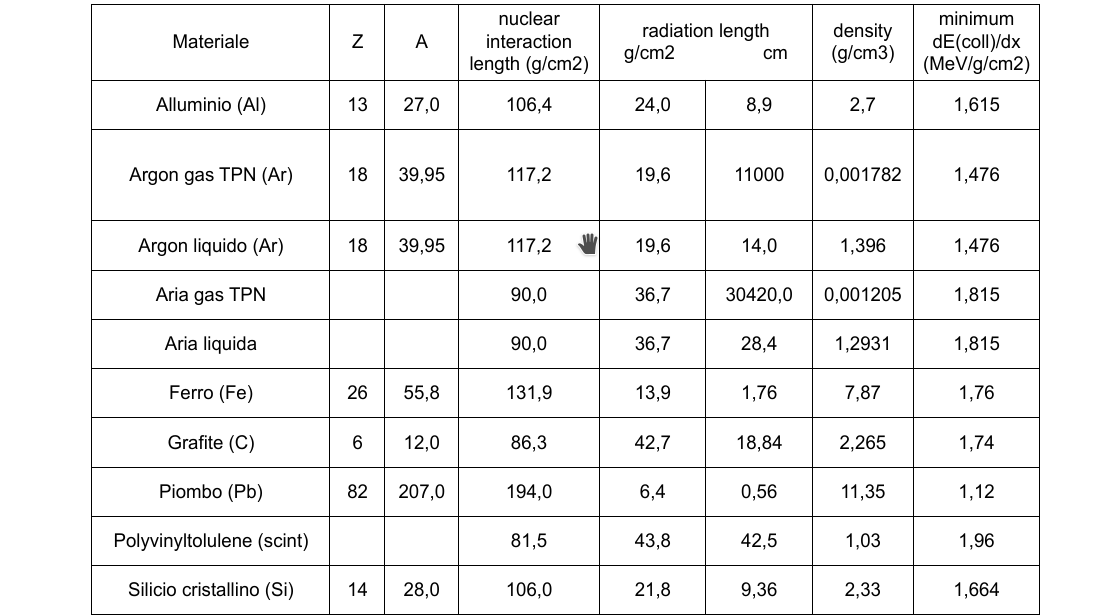
\includegraphics[width=0.8\textwidth]{immagini/materials.png}
	\caption{Tabella con proprietà di alcuni materiali.}
	\label{fig:}
\end{figure}

Dobbiamo ripassare, quantità per quantità, tutte le cose che ci serviranno sulle particelle:

\paragraph{Energia persa per irraggiamento}%
Questa è trascurabile per tutti tranne che per gli elettroni. Per questi ultimi dobbiamo distinguere tra elettroni aventi energia maggiore o minore dell'energia critica:
\[
	E_{c} \approx 98 \frac{\text{MeV}}{Z^{1 /3}}
.\] 
Se gli elettroni hanno una energia maggiore di quest'ultima allora si applica 
\[
	E_{\text{irr}}= E_0 e^{- x /X_0}
.\]
Altrimenti potremmo dare una stima dell'energia irraggiata mediante la formula per uno  schermaggio incompleto come spiegato sul Jackson, ma la risposta sarà comunque che questa energia è trascurabile rispetto a quella persa per collisioni.

\paragraph{Energia persa per collisioni}%
Se l'energia persa per irraggiamento è trascurabile è pratico vedere se l'energia con cui il proiettile incide è sufficiente ad attraversare il materiale.\\
Per far questo è necessario utilizzare \href{https://www.nist.gov/pml/stopping-power-range-tables-electrons-protons-and-helium-ions}{i dati ed i grafici} sullo stopping range dal PDG, una volta messi i parametri ed ottenuta la curva di Range si effettuano i seguenti passaggi:
\begin{itemize}
	\item Determinare il Range in ingresso $R\left( E_{\text{in}}\right)$ graficamente.
	\item Calcolare il Range di uscita come $R\left( E_{\text{out}} \right)= R\left( E_{\text{in}} \right) - \Delta x$.
	\item Determinare $E_{\text{out}}$ sulle $x$ in corrispondenza di $R\left( E_{\text{out}} \right)$,
\end{itemize}
Se l'energia trovata risulta graficamente prossima allo zero allora l'energia persa per collisioni è tutta l'energia incidente.\\
Se si ha invece una energia persa per irraggiamento non trascurabile rispetto all'energia in ingresso allora si applica la formula di Tsai approssimata come nella \hyperref[sec:4.b.16]{Domanda 4.b.16}.
\paragraph{Probabilità di interazione forte}%
Questa interazione avviene soltanto per adroni, quindi nel nostro caso il $\pi^{-}$ ed il $p$. Per queste particelle si calcola la sezione d'urto nucleare come l'area della circonferenza avente raggio la somma del raggio del proiettile e del raggio del nucleo bersagio:
\[
	\sigma=\pi\left( r_{p}+R \right)^2 = \pi\left( 1.25 + 1.25\cdot A^{1/3} + 2 \right)^2 \text{ fm}^2 
.\] 
successivamente il conto da fare è:
\[
	P_{\text{forte}}= \sigma \frac{\rho N_{A}}{A}x
.\] 
\paragraph{Angolo quadratico medio di multiplo scattering}%
Se la particella riesce ad uscire il conto da effettuare è quello della \hyperref[sec:4.b.18]{Domanda 4.b.18}

\subsection[]{Per un muone che attraversi, incidendo perpendicolarmente, una lastra di Ferro di 5cm di spessore in cui e' presente un campo magnetico di intensita' nota, calcolare il valore numerico del rapporto fra la deflessione angolare dovuta al campo magnetico e la dispersione quadratica media dovuta al multiplo scattering. Come sara’ la funzione di distribuzione dell’angolo in uscita? Quale e’ la dipendenza dall’energia del muone incidente?
}
\label{sec:4.b.20}
Ipotizziamo che l'energia del muone sia tale da garantire che oltrepasserà la lastra (possiamo tornarci dopo) e che la frazione di energia persa nella lastra sia molto inferiore dell'energia iniziale in modo da considerare la curvatura magnetica uniforme.\\
Calcoliamo per prima cosa il raggio di curvatura dovuto al solo campo magnetico:
\[
	R= \frac{mv}{eB}= \frac{P}{e B} = \frac{3}{10} \frac{P  \text{ [GeV/c]}}{B \text{ [T]}}
.\] 
Dove si è utilizzato l'esoterica conversione della carica elementare in unità gaussiane. Con un pò di geometria si calcola il seno dell'angolo di deflessione magnetic:
\[
	\sin\theta_{\text{m}}= \frac{x}{R} = \frac{50}{3} \cdot 10^{-3}\text{ [m]}  \frac{B \text{ [T]}}{P  \text{ [GeV/c]}}
.\] 
Approssimando adesso angoli piccoli (è necessario che $ \frac{P \text{ [GeV/c]}}{B \text{ [T]}}>\sim 1$ ) si ottiene:
\[
	\theta_{\text{m}}= \frac{x}{R} \approx 15 \text{ mrad}  \frac{\text{ [m] } B \text{ [T]}}{P  \text{ [GeV/c]}}
.\] 
Per l'angolo quadratico medio di multiplo scattering si ha invece:
\[
	\theta_0= \frac{13.6 \text{ [MeV]}}{PV} \sqrt{ \frac{5 \text{ [mm]}}{X_0}} 
.\] 
Nel ferro si ha $X_0 = 1.76$ cm, inoltre possiamo assumere $\beta \sim 1$ per la nostra stima, quindi:
\[
	\theta_0 \approx \frac{13.6 \cdot 10^{-3} \text{ [eV]}}{P \text{ [GeV/c] [m/s]}} \sqrt{ \frac{5 \cdot 10^{-3}\text{ [m]} }{1.76 \cdot 10^{-2}\text{ [m]}}}
	\approx 7.24 \text{ mrad} \cdot \frac{\text{[eV]}}{P\text{ [GeV/c] [m/s]} }
.\] 
Quindi il rapporto cercato (sempre per impulsi sufficienti a garantire l'uscita del muone e angoli di deflessione piccoli) è indipentente dall'impulso:
\[
	\frac{\theta_{m}}{\theta_0 \sqrt{2}} \approx 0.3\cdot B \text{ [T]}
.\]
La distribuzione angolare sarà in tal caso una Moliere centrata in $\theta_{m}$.

\subsection[]{Cercando i dati nelle apposite figure o tabelle si calcolino il valore (o i limiti) dell'energia degli elettroni emessi nello stato finale della reazione $\gamma$+C per energie del fotone incidente pari a: 1keV, 10keV, 100keV, 1MeV, 10MeV.
}
\label{sec:4.b.21}
La sezione d'urto di un fotone sull'atomo di carbonio segue questi andamenti:
\begin{figure}[H]
	\centering
	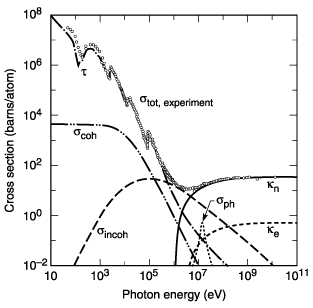
\includegraphics[width=0.6\textwidth]{immagini/cross-section-photon.png}
	\caption{Sezione d'urto di fotone su carbonio.}
	\label{fig:immagini-cross-section-photon-png}
\end{figure}
Ad 1 keV il processo dominante è il fotoelettrico. Per questo processo l'energia cinetica dell'elettrone prodotto è la stessa l'energia del fotone incidente (trascurando l'energia di legame dell'ordine di 1-10 eV). \\
A 10 keV domina ancora il fotoelettrico ma iniziano ad essere importanti anche il Rayleigh ($\sigma_{coh}$ in figura) ed il compton ($\sigma_{incoh}$ in figura).
Nel primo (che è uno scattering elastico) l'elettrone non acquista energia. Nel secondo invece l'energia dell'elettrone è compresa tra gli 0 ed i 9 keV a seconda dell'angolo di scattering:
\[
	E_{phot} = \hbar\omega= \frac{h}{\lambda}c 
.\] 
Il cambio di frequenza del Compton è noto e vale 
\[
	\Delta \lambda = \lambda'\left( 1-\cos\theta \right) 
.\] 
Con $\lambda' = 2.43$pm lunghezza d'onda Compton.\\
La lunghezza d'onda iniziale vale: $\lambda = hc /E = hc /10$keV$\approx 20$ pm. Qunidi al massimo questa può diventare $\lambda_{\text{fin}} = \lambda + 2\lambda'$ se l'urto è centrale. L'energia minima del fotone dopo l'urto è quindi:
\[
E^{\text{Compton}}_{\text{min}}= \frac{h}{\lambda_{\text{fin}}}c = \frac{\frac{197}{2\pi}\text{MeV}\cdot\text{fm}}{24.86 \text{pm}} \approx 1.3 \text{ keV}
.\] 
Per differenza (conservazione dell'energia) si ottiene che l'elettrone può avere energia massima di $E^{\text{el}}_{\text{max}} \approx 8.7$ keV, l'energia mininima si ha quando il coseno vale 1 e quindi la lunghezza d'onnda del fotone non cambia. In tal caso $E^{\text{el}}_{\text{min}}=0$.\\
A 100 keV ed a 1 MeV il dominante è il Compton mentre a 10 MeV inizia ad essere importante la produzione di coppie.
Per la produzione di coppie trascurando il rinculo del nucleo ci si aspetta che ciascuno dei prodotti abbia energia di circa 5 MeV.

\subsection[]{Ricavare la relazione tra angolo di scattering e cambio di frequenza nell'effetto Compton
}
\label{sec:4.b.22}
Definiamo k e k' i vettori d'onda del fotone prima e dopo l'urto e p, p' il 4-impulso dell'elettrone prima e dopo l'urto. Dalla comservazione del quadrimpulso si deve avere che:
\[
	\hbar\left( k- k \right)= p'-p	
.\] 
Facendo la norma quadra a destra e sinistra e ricordando che l'elettrone è comsiderato inizialmente fermo si ottiene:
\[
	2\hbar\left( 0 + 0 - 2\left( \omega\omega'- kk'\cos\theta\right) \right) = m^2+m^2- 2mE'
.\] 
In cui $\theta$ è l'angolo di scattering. Adesso sfruttiamo la conservazione dell'energia ($E' = \hbar\omega + m - \hbar\omega'$) per ottenere:
\[
	\frac{2\hbar\omega\omega'}{c}\left( 1-\cos\theta \right) = 2m_{e}c^2\hbar\left( \omega-\omega' \right) 
.\] 
Se passiamo alle lunghezze d'onda otteniamo la relazione cercata:
\[
	\Delta \lambda = \lambda_{c}\left( 1-\cos\theta \right) 
.\] 
Dove $\lambda_{c}= \frac{h}{m_{e}c}$ 



\subsection[]{Cercando i dati delle sezioni d’urto totali nelle apposite figure o tabelle (reperibili anche nella compilazione Particle Data Group http://pdg.lbl.gov ) si calcoli la probabilità di interazione di:\\
• un fotone da 100 eV che incida su 1 $\mu$m di grafite\\
• un fotone da 1 MeV che incida su 1 mm di grafite\\
• un fotone da 10 MeV che incida su 1 mm di Piombo\\
• un fotone da 50 KeV che incida su 1 $\mu$m di Piombo\\
• un neutrino da 100 GeV che incida su 1 km di grafite\\
• un protone da 100 GeV che incida su 1 cm di grafite\\
}
\label{sec:4.b.23}
Partiamo dal metodo da adottare: la probabilità cercata è data da
\[
	P = n_{s}\sigma
.\] Dove $n_{s}$ è la densità superficiale di bersagli. Questa quantità può essere espressa in funzione di variabili tipiche del materiale:
\[
	P = \frac{\rho}{A \text{[g]}}N_{A}L\sigma
.\] 
\subsection[]{Esprimere la sezione d'urto Rayleigh in funzione della sezione d'urto differenziale Thomson e del fattore di forma atomico F($\theta$).
}
\label{sec:4.b.24}
La sezione d'urto Rayleigh differenziale vale
\[
	\frac{\mbox{d} \sigma_{el}}{\mbox{d} \Omega}= \left.\frac{\mbox{d} \sigma_{el}}{\mbox{d} \Omega} \right|_{e} \left| Z F\left( \bs{q} \right)  \right|^2 \quad
		\text{ con }
	\quad
	\left.\frac{\mbox{d} \sigma_{el }}{\mbox{d} \Omega} \right|_{e}= 
		\frac{r_e^2\omega^4}{\left( \omega_0^2-\omega^2 \right)^2 + \omega^2\Gamma_{tot}^2\left( \omega \right)} \frac{1+\cos^2\theta}{2}
.\] 

Per ottenere quanto richiesto dal testo è necessario integrare sull'angolo solido e conoscere il fattore di forma dipendente dall'angolo di scattering $\theta$.

\subsection[]{Dimostrare, utilizzando il materiale distribuito, perchè nell’esperimento di Anderson sulla scoperta del positrone alcune tracce positive osservate non
possono essere nessuna delle particelle positive conosciute nel 1932.
}
\label{sec:4.b.25}
Riprendendo la trattazione della \hyperref[sec:4.a.34]{Domanda 4.a.34} l'impulso iniziale misurato da Anderson era $p_{i}= 63$ MeV/c, quello finale invece era $p_{f}=22.5$ MeV/c, se fosse stato un protone (unica particella con quella carica positiva conosciuta allora) sarebbe stato:
\[
	E_{i}= \frac{p^2}{2m_{p}}\approx 2.1 \text{ MeV}
.\] 
Un protone con quella energia ha un range in aria di circa $7$ mm, la traccia della foto di Anderson è lunga almeno $30$ cm, per questo non poteva essere un protone.


\subsection[]{Calcolare la velocità media dei pioni e antiprotoni nell'esperimento di Segrè (quantità di moto 1.19 Gev/c) dopo che hanno attraversato il contatore Cherenkov a quarzo (spessore 2.5", densità relativa 2.2).
}
\label{sec:4.b.26}
Per il calcolo possiamo utilizzare lo spessore relativo del materiale: 
\[
	\Delta x = x \text{ [pollici]}\cdot \rho_{rel}= (2.5 \ \cdot \ 2.54) \text{ [cm]} \ \cdot \ 2.2 \left[\text{g}/\text{cm}^3 \right] = 13.9\left[\text{g}/\text{cm}^2 \right]
\]
L'energia dell'antiprotone entrante è 
\[
	E_{\overline{p}} = \sqrt{ p_{in}^2+m_{p}^2} \approx 1.51 \text{ GeV}
.\] 
Da cui l'energia cinetica: $T_{\overline{p}}= E_{\overline{p}}-m_{p}= 0.57$ GeV.\\
Lo stopping power per tale energia e per il diossido di silicio (quarzo) vale $dE /dx = 2.17$ MeV cm$^2$/g, da questo si ricava l'energia finale:
\[
	\Delta E = \frac{\mbox{d} E}{\mbox{d} x} \Delta x \approx 30.1 \text{ [MeV]} \implies T_{f} \approx 0.54 \text{ [GeV]}
.\] 
Quindi tornando indietro con le formule inverse si ricava che:
\[
	E_{f} = 1.48 \text{ GeV} = m_{p}\gamma = m_{p}\sqrt{\frac{1}{1-\beta^2}} 
.\] 
Quindi:
\[
	\beta = \sqrt{1 - \left( \frac{m_{p}}{E_{f}} \right)^2} \approx 0.773 
.\] 
Analogamente si può procedere per i pioni se solo esistessero le dannate tabelle.



